\documentclass[pdflatex,compress]{beamer}

\usetheme[darktitle,framenumber,totalframenumber]{UniversiteitAntwerpen}
%\usetheme[light,framenumber,totalframenumber]{UniversiteitAntwerpen}

\usefonttheme[onlymath]{serif}
\usepackage{lipsum}
\setbeamertemplate{caption}[numbered]
\beamertemplatenavigationsymbolsempty



\title{Presentation for Bachelor Thesis}
%\subtitle{This is a dummy subtitle}

\author{Bernhard Gstrein}

\begin{document}

\maketitle

\AtBeginSection[]{}
\section{Introduction / Motivation (4 min)}

\begin{frame}
\frametitle{Introduction}
\begin{itemize}
	\item Materials with certain properties $\rightarrow$ How do we find them?
		\begin{itemize}
			\item Na{\"i}ve approach: Dig for it in the earth
			\item More systematic: Create them ourselves
		\end{itemize}
	\item Need to understand underlying physical processes better $\rightarrow$ Simulate a solid
		\begin{itemize}
		\item Analog: Arrange atoms in lattice in the lab $\rightarrow$ Most promising for now
		\item Digital: On a computer $\rightarrow$ Limitations of classical computers, quantum computers won't be there in the near future
		\end{itemize}
\end{itemize}
\end{frame}

\begin{frame}
\frametitle{Introduction}
\begin{itemize}
	\item Before any experiment: Theoretical model needed
\end{itemize}
Our goal:
\begin{itemize}
	\item Establish a theoretical model arranging atoms in a lattice
	\item Check validity of that model with simulations
\end{itemize}
\end{frame}

\begin{frame}
\frametitle{Table of Contents}
\tableofcontents
\end{frame}

\AtBeginSection[]
{
  \begin{frame}
    \frametitle{Table of Contents}
    \tableofcontents[currentsection]
  \end{frame}
}

\section{Setting up our model (9 min)}

\begin{frame}
\frametitle{Creating an artificial solid}
\begin{columns}
\column[T]{0.5\textwidth}
How do we make atoms arrange in a lattice pattern?
\begin{itemize}
	\item Two counter-propagating laser beams, $\omega_\text{l} << \omega_\text{a}$
	\item Optical cavities: Coerce atoms into creating their own trapping potential
	\item Light and atoms: Composite system $\psi_\text{total} = \psi_\text{light} \otimes \psi_\text{atom}$
\end{itemize}
\column[T]{0.5\textwidth}
\begin{figure}
\centering
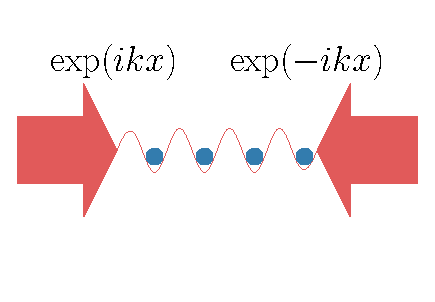
\includegraphics[width=.6\textwidth]{images/counter_propagating.eps}
\vspace*{-5mm}
\caption{Counter-propagating lasers.}
\end{figure}
\vspace{-1.5em}
\begin{figure}
\centering
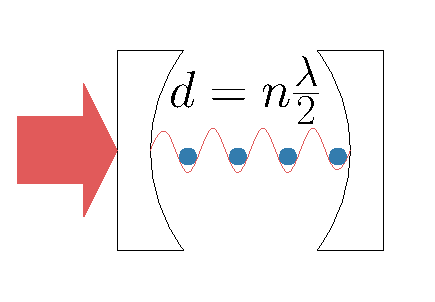
\includegraphics[width=.6\textwidth]{images/cavity.eps}
\vspace*{-5mm}
\caption{Optical cavity.}
\end{figure}
\end{columns}
\end{frame}

\begin{frame}
\frametitle{Cold atoms in cavities}
\begin{itemize}
	\item Problem: Motion of one atom affects cooling of another
	\item Solution: Transversal pumping
\end{itemize}
Paper: Collective Cooling and Self-Organization of Atoms in a Cavity \cite{domokos2002}
\vspace{-2em}
\begin{columns}
\column{0.5\textwidth}
\begin{figure}
\centering
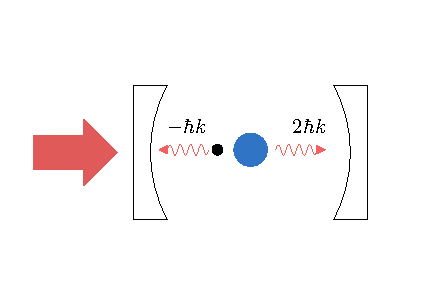
\includegraphics[width=1\textwidth]{images/pump_long.eps}
\caption{Longitudinal pump.}
\end{figure}
\column{0.5\textwidth}
\begin{figure}
\centering
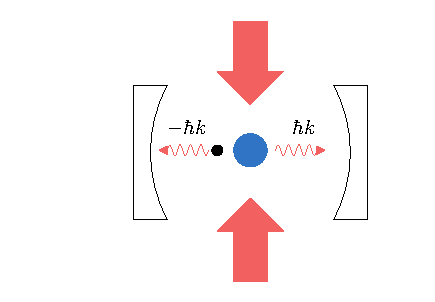
\includegraphics[width=1\textwidth]{images/pump_trans.eps}
\caption{Transversal pump.}
\end{figure}
\end{columns}
\end{frame}

\begin{frame}
\frametitle{The Hamiltonians}
Longitudinal pump ($\lambda / 2$-periodic):
\begin{align}
H_\text{long} = \frac{p^2}{2m} + V_\text{ext}(x) - \hbar \Delta_\text{c} a^\dagger a + \hbar \eta (a + a^\dagger) + \hbar U_0 \cos(kx)^2 a^\dagger a
\end{align}Transversal pump ($\lambda$-periodic):
\begin{align}
\begin{split}
H_\text{transv} = \frac{p^2}{2m} + V_\text{ext}(x) - \hbar \Delta_c a^\dagger a + \hbar \eta \cos(kx) (a + a^\dagger) + \\
 + \hbar U_0 \cos(kx)^2 a^\dagger a
\end{split}
\end{align}
\end{frame}

\begin{frame}
\frametitle{Transversal pump: Superposition}
When we do simulations we obtain a superposition of two symmetric states
\begin{columns}
\column{0.5\textwidth}
\begin{figure}
\centering
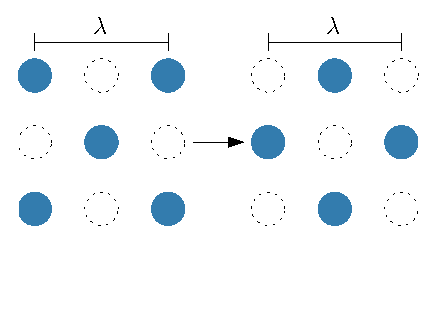
\includegraphics[width=1\textwidth]{images/lattice_drawing.eps}
\vspace*{-10mm}
\caption{Lattice.}
\end{figure}
\column{0.5\textwidth}
\begin{figure}
\centering
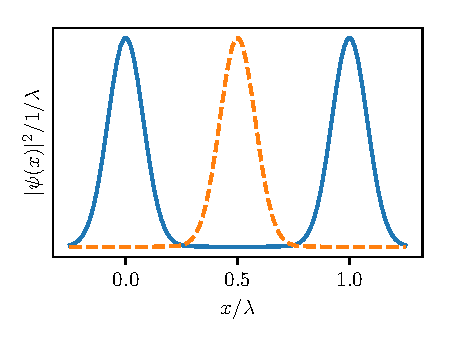
\includegraphics[width=1\textwidth]{images/density_superposition.pdf}
\vspace*{-10mm}
\caption{Wave function densities.}
\end{figure}
\end{columns}
\end{frame}

\begin{frame}
\frametitle{Our expectations}
Paper: Self-organization of a Bose-Einstein condensate in an optical cavity \cite{Nagy2008}
\begin{columns}
\column{0.5\textwidth}
\begin{figure}
\centering
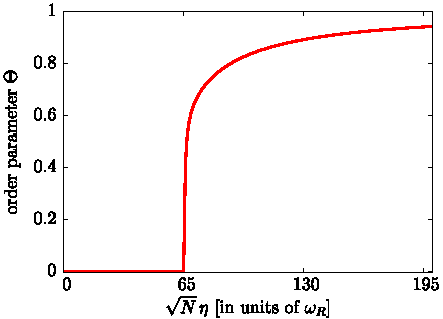
\includegraphics[width=1\textwidth]{images/domokos_order_parameter.pdf}
\caption{Order parameter.}
\end{figure}
\column{0.5\textwidth}
\begin{figure}
\centering
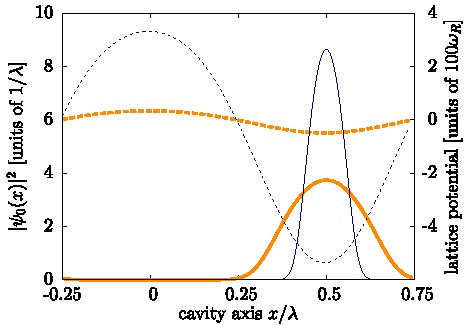
\includegraphics[width=1\textwidth]{images/domokos_lattice_potential.pdf}
\caption{Lattice potential.}
\end{figure}
\end{columns}
\end{frame}

\begin{frame}
\frametitle{Our expectations}
\begin{itemize}
	\item Atoms are localized in "valleys" of optical potential
	\item Momenta:
		\begin{itemize}
			\item Longitudinal: $p = 2 n \hbar k$
			\item Transversal: $p = n \hbar k$
		\end{itemize}
	\item The more we pump, the more photons we will get
	\item Abrupt self-organization with transversal pumping
\end{itemize}
\end{frame}

\section{Setting up the simulation (4 min)}

\begin{frame}
\frametitle{The Julia language and QuantumOptics.jl}
\begin{itemize}
	\item High-performance languages like C, Fortran cumbersome to program
	\item Julia: high level convenience, low-level performance \cite{julialang}
	\item How to program it into computer?
	\begin{itemize}
		\item Starting from scratch: redundant
		\item More convenient: QuantumOptics.jl: Quantum optics simulation framework \cite{qojulia}	
	\end{itemize}
\end{itemize}
\end{frame}

\begin{frame}
\frametitle{Code snippet: Longitudinal pump}
\vspace{-2em}
\begin{figure}
\centering
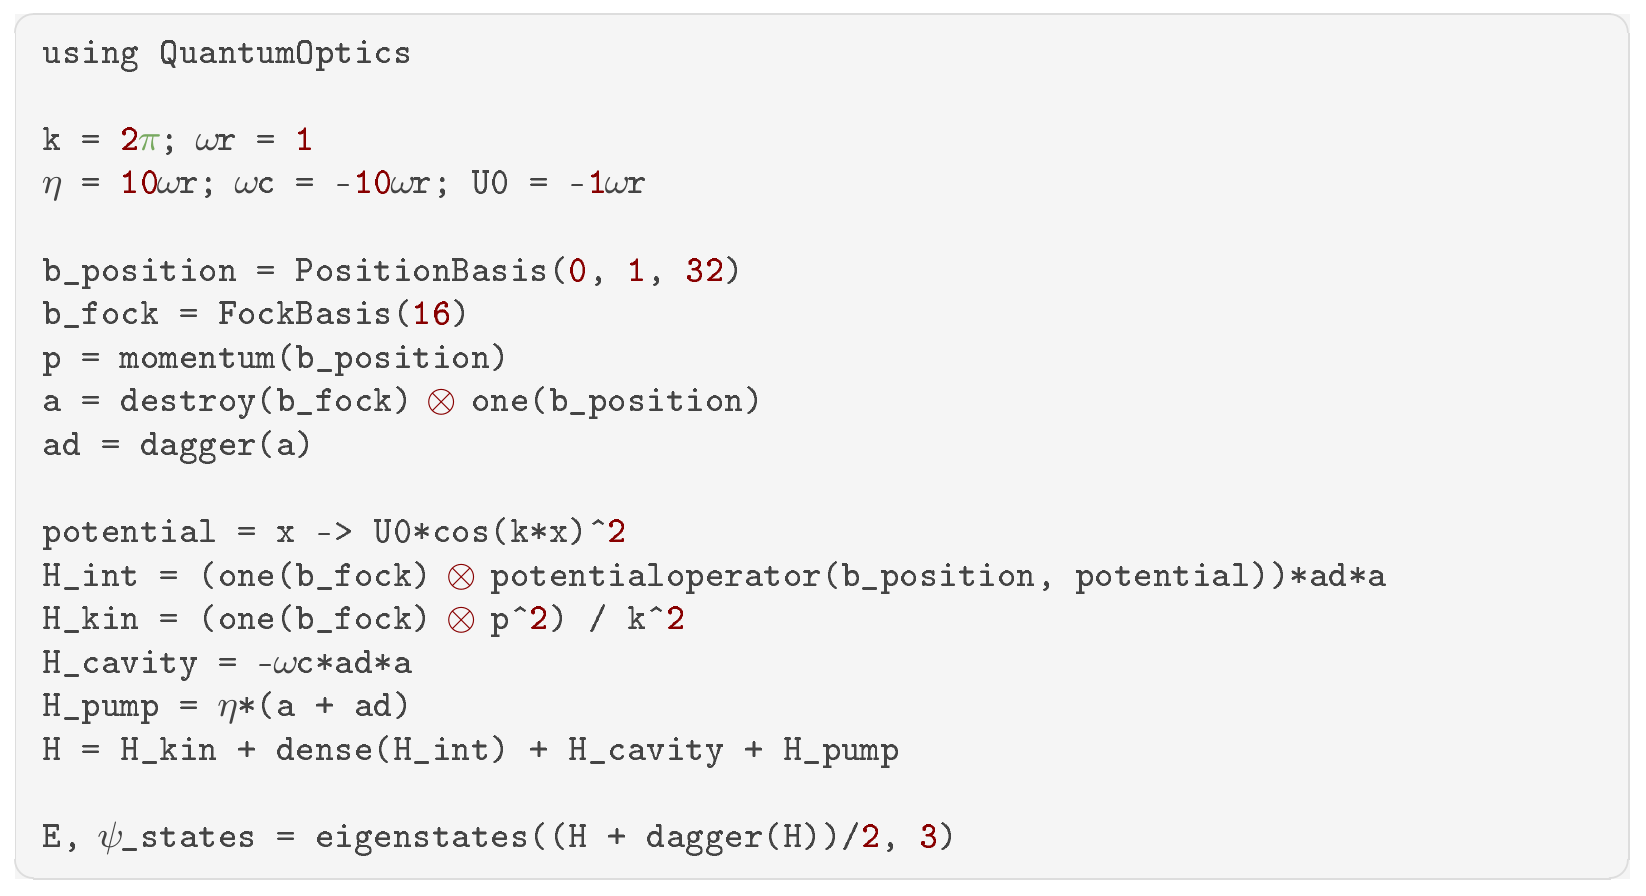
\includegraphics[width=1\textwidth]{images/code_screenshot.png}
\end{figure}
\end{frame}

\section{Results and Discussion (10 min)}


\begin{frame}
\frametitle{Position wave function densities}
\vspace{-1em}
\begin{figure}
\centering
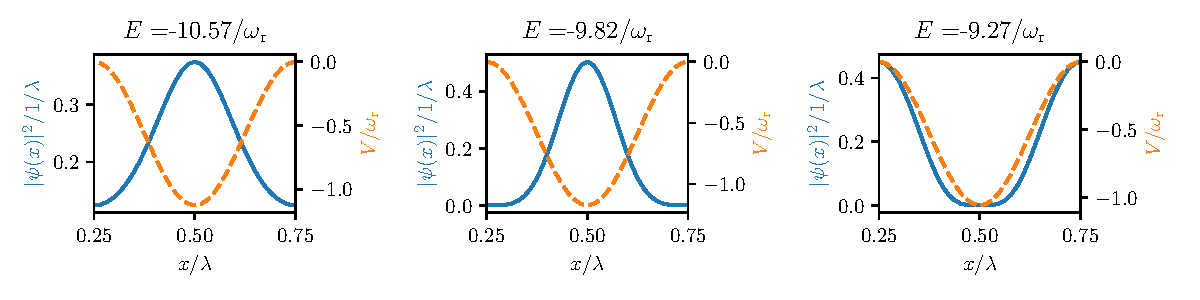
\includegraphics[width=1\textwidth]{images/dens_long.pdf}
\vspace*{-7mm}
\caption{Longitudinal.}
\end{figure}
\vspace{-1em}
\begin{figure}
\centering
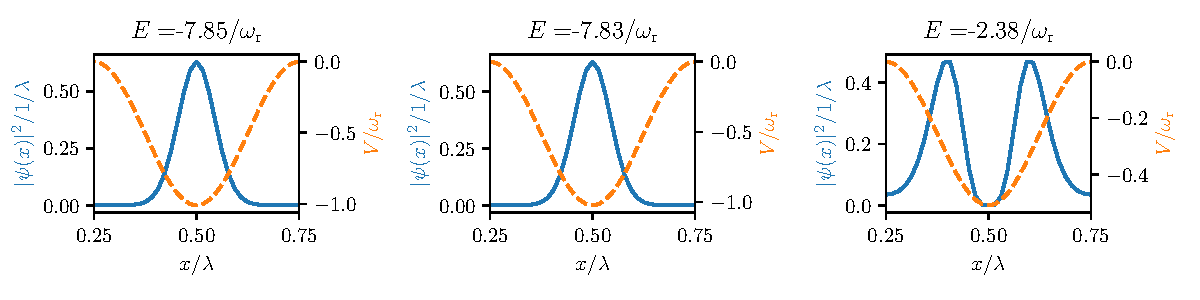
\includegraphics[width=1\textwidth]{images/dens_trans.pdf}
\vspace*{-7mm}
\caption{Transversal.}
\end{figure}
\end{frame}

\begin{frame}
\frametitle{Components of the wave function}
\vspace{-3em}
\begin{align}
\psi(k) & = \frac{1}{N} \sum_l c_l \exp(likx) =  \\
& = \frac{1}{N} \Big( c_0 + c_{\pm 1} \exp(ikx) + c_{\pm 2} \exp(2ikx) + \dots \Big) \nonumber
\end{align}
\vspace{-1em}
\begin{table}[!htb]
\centering
\begin{tabular}{lll}
$c_l$    & wave number & momentum    \\
\hline \\
$c_0$    & 0           & 0           \\
$c_{\pm 1}$ & $k \rightarrow \exp(ikx)$         & $\hbar k$   \\
$c_{\pm 2}$ & $2k \rightarrow \exp(2ikx)$        & $2 \hbar k$ \\
$c_{\pm 3}$ & $3k \rightarrow \exp(3ikx)$        & $3 \hbar k$ \\
$\vdots$ &             &            
\end{tabular}
\caption{Wave function coefficients.}
\end{table}
\end{frame}

\begin{frame}
\frametitle{Momentum distribution}
\vspace{-1em}
\begin{figure}
\centering
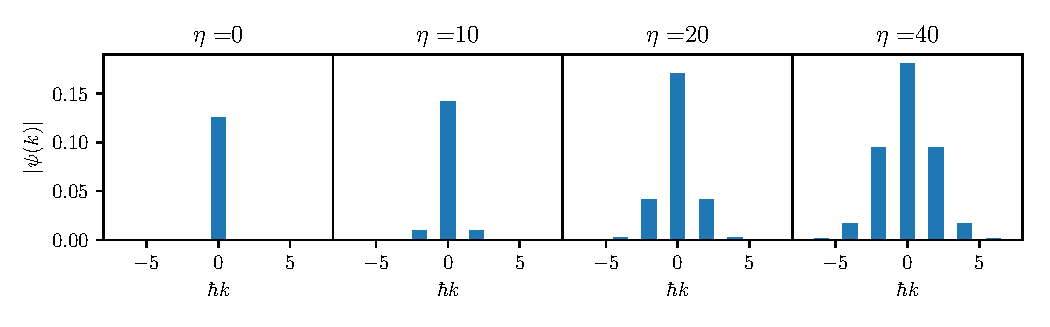
\includegraphics[width=.9\textwidth]{images/mom_long.pdf}
\vspace*{-6mm}
\caption{Longitudinal.}
\end{figure}
\vspace{-2em}
\begin{figure}
\centering
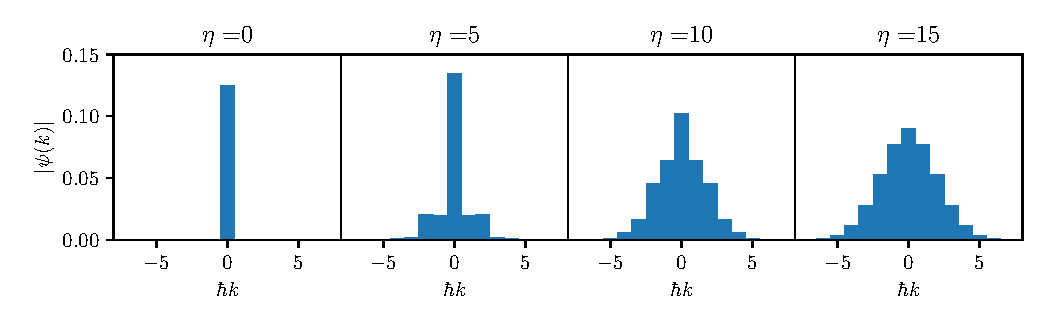
\includegraphics[width=.9\textwidth]{images/mom_trans.pdf}
\vspace*{-6mm}
\caption{Transversal.}
\end{figure}
\end{frame}

\begin{frame}
\frametitle{Photon number distribution}
\vspace{-1em}
\begin{figure}
\centering
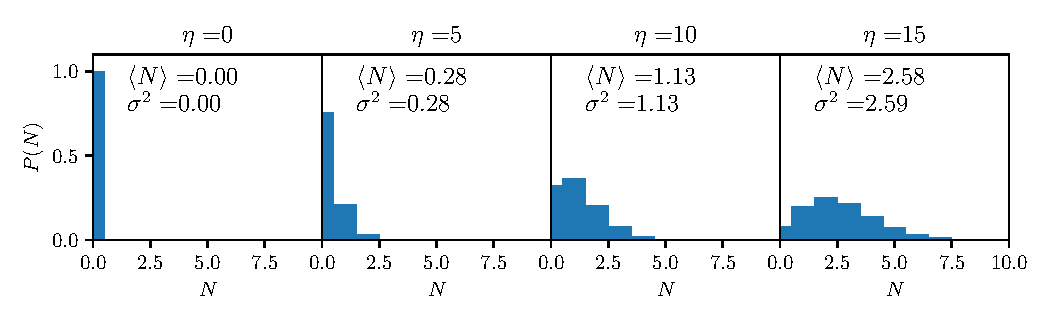
\includegraphics[width=.9\textwidth]{images/pho_dens_long.pdf}
\vspace*{-6mm}
\caption{Longitudinal.}
\end{figure}
\vspace{-2em}
\begin{figure}
\centering
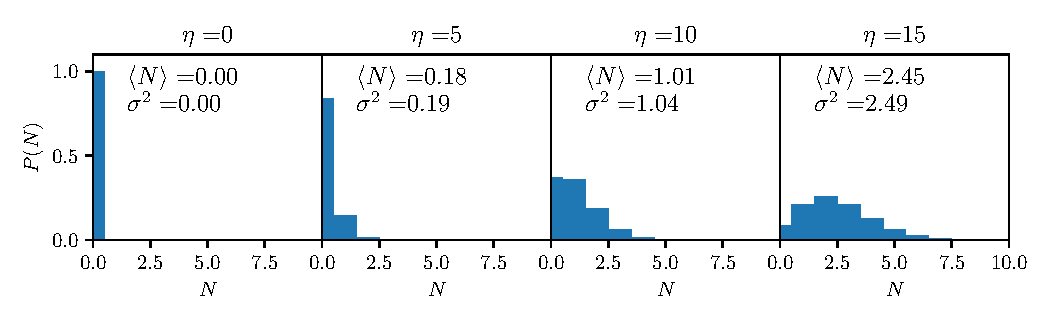
\includegraphics[width=.9\textwidth]{images/pho_dens_trans.pdf}
\vspace*{-6mm}
\caption{Transversal.}
\end{figure}
\end{frame}

\begin{frame}
\frametitle{Husimi Q representation}
\vspace{-1.5em}
\begin{figure}
\centering
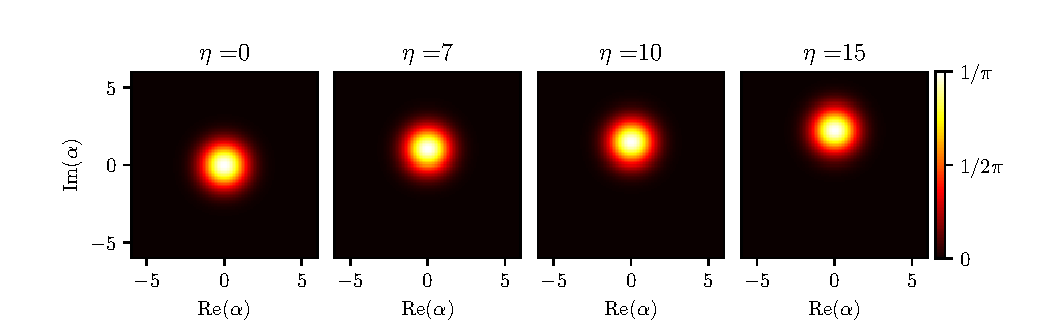
\includegraphics[width=.9\textwidth]{images/qfunc_long.pdf}
\vspace*{-3mm}
\caption{Longitudinal.}
\end{figure}
\vspace{-2em}
\begin{figure}
\centering
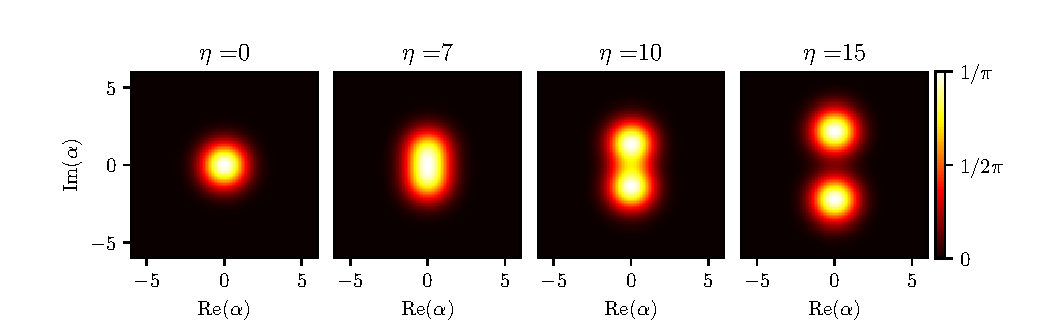
\includegraphics[width=.9\textwidth]{images/qfunc_trans.pdf}
\vspace*{-3mm}
\caption{Transversal.}
\end{figure}
\end{frame}

\begin{frame}
\frametitle{Breaking the symmetry}
\begin{columns}
\column{0.5\textwidth}
\begin{figure}
\centering
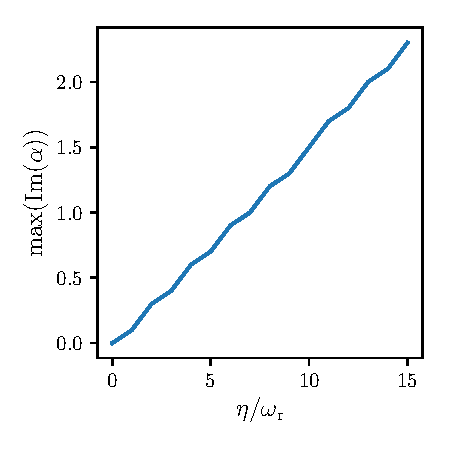
\includegraphics[width=1\textwidth]{images/theta_long.pdf}
\vspace*{-10mm}
\caption{Longitudinal.}
\end{figure}
\column{0.5\textwidth}
\begin{figure}
\centering
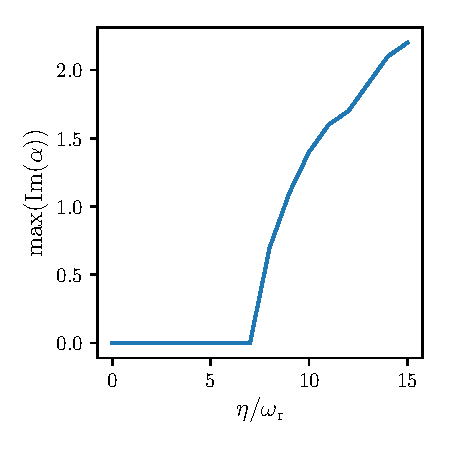
\includegraphics[width=1\textwidth]{images/theta_trans.pdf}
\vspace*{-10mm}
\caption{Transversal.}
\end{figure}
\end{columns}
\end{frame}

\section{Recap / Conclusion (2 min)}

\begin{frame}
\frametitle{Recap}
What we discussed in this presentation...
\begin{itemize}
	\item Why are we doing quantum simulations and how
		\begin{itemize}
			\item Most promising for now: Analog quantum simulations
		\end{itemize}
	\item Arrange atoms in lattice to simulate solid
		\begin{itemize}
			\item Use laser to trap atoms
			\item Make use of cavity
			\item Transversal pumping
		\end{itemize}
	\item Does our theoretical model make sense $\rightarrow$ Simulations
		\begin{itemize}
			\item Atoms localized in "valleys" of potential
			\item Specific momenta with longitudinal, transversal pump
			\item More pumping $\rightarrow$ More photons
			\item Abrupt self-organization with transversal pumping
		\end{itemize}
\end{itemize}
\end{frame}

\section{Special Thanks (1 min)}

\begin{frame}
\frametitle{Special Thanks}
\begin{center}
\huge Helmut Ritsch \\
\small for Opportunity, Subject \\
\vspace{2em}
\huge Stefan Ostermann \\
\small for Guidance, Discussion
\end{center}
\end{frame}

\begin{frame}
\begin{center}
\huge Thank You!
\end{center}
\end{frame}

\section{References}

\begin{frame}[allowframebreaks]
\bibliographystyle{unsrt}
\bibliography{bibliography}
\end{frame}

\end{document}